%************************************************
\chapter{Motivación e Introducción}\label{ch:introduction}
%************************************************

\listoftodos[TODO list]

\todo[inline]{Pipeline Genérico, detallar cada parte, con ejemplos y
  justificación}

\todo[inline]{Pipeline Específico, con paquete real (CoreNLP), explicar de forma
  breve cada parte, inglés)}

\todo[inline]{Desribir de forma más detallada el Dep Parsing, mencionar state of
  the art (3/4 papers), entre ellos el implementado}

\todo[inline]{Sección con algoritmo implementado, reiterando sección anterior
  pero con lujo de detalles (Teóricos y código)}

\todo[inline]{Motivación: Falta de software español, justificar decisión de
  afrontar problema.}

\info{Añadir sección ``\emph{El resto del paper está organizado\dots}''}

\section{¿Qué es el Procesamiento del Lenguaje Natural?}
\label{sec:whatisnlp}

El lenguaje natural se refiere a cualquier lenguaje hablado por un humano, (\eg
Inglés, Castellano o Chino). El \acfi{NLP}\acused{NLP}\graffito{\acf{PNL}} es un
campo de la ciencia de la computación e ingeniería desarrollado a partir del
estudio del lenguaje y la computación lingüistica dentro del campo de la
\ac{IA}. Los objetivos del \ac{NLP} son diseñar y construir aplicaciones que
faciliten la interacción humana con la máquinas y otros dispositivos mediante el
uso del lenguaje natural. Dentro del amplio campo del \ac{NLP} podemos
distinguir las siguientes áreas principales:

El lenguaje natural se refiere a cualquier lenguaje hablado por un humano, (\eg
Inglés, Castellano o Chino). El \ac{NLP}\graffito{\acf{PNL}} es un campo de la
ciencia de la computación e ingeniería desarrollado a partir del estudio del
lenguaje y la computación lingüistica dentro del campo de la \ac{IA}. Los
objetivos del \ac{NLP} son diseñar y construir aplicaciones que faciliten la
interacción humana con la máquinas y otros dispositivos mediante el uso del
lenguaje natural. Dentro del amplio campo del \ac{NLP} podemos distinguir las
siguientes áreas principales:

\paragraph{Resúmenes} este área incluye aplicaciones que puedan, basándose en
una colección de documentos, dar como salida un resumen coherente del contenido
de los mismos. Otra de las posibles aplicaciones sería generar presentaciones a
partir de dichos documentos. En los últimos años, la información disponible en
la red ha aumentado considerablemente. Un claro ejemplo es la literatura
científica, o incluso repositorios de información más genérica como
\emph{Wikipedia}. Toda esta información escrita en lenguaje natural puede
aprovecharse para entrenar modelos que sean capaces de generar hipótesis por sí
mismos, generar resúmenes o extraer hechos. Un ejemplo claro puede ser la
extracción de hechos básicos que relacionen dos entidades (\emph{``Luís es padre
de Cristina''}.

\paragraph{Traducción automática:} Esta fue la principal área de investigación
en el campo del \ac{NLP}. Como claro ejemplo tenemos el traductor de Google,
mejorando día a día. Sin embargo, un traductor realmente útil sería aquel que
consiga traducir en tiempo real una frase que le dictemos mientras decidimos qué
línea de autobús debemos coger para llegar a tiempo a una conferencia en
Zurich. La traducción entre lenguajes es quizá una de las formas más
transcendentales en las que las máquinas podrían ayudar en comunicaciones entre
humanos. Además, la capacidad de las máquinas para traducir entre idiomas
humanos se considera aún como un gran test a la \ac{IA}, ya que una traducción
correcta no consiste en el mero hecho de generar frases en un idioma humano,
también requiere del conocimiento humano y del contexto, pese a las ambigüedades
de cada idioma. Por ejemplo, la traducción literal
\improvement[fancyline]{Debería buscar algún ejemplo más claro?}%
\emph{``bordel''} en Francés significa Burdel; pero si alguien dice \emph{``Mi
  cuarto es un burdel''}, el traductor debería tener el conocimiento suficiente
para inferir que la persona se está refiriendo a que su habitación es un
desorden.

La traducción automática fue una de las primeras aplicaciones no numéricas de la
computación y comenzó a estudiarse de forma intensiva en la década de los
50. Sin embargo, no fue hasta la década de los 90 cuando se produjo una
tansformación en este área. IBM se hizo con una gran cantidad de frases en
Inglés y Francés que eran traducciones las unas de las otras, \graffito{Conocido
como texto paralelo} lo cual permitió recopilar estadísticas de traducciones de
palabras y secuencias de palabras, concediento así el desarrollo de modelos
probabilísticos para la traducción automática. Hasta ese momento, todo el
análisis gramático se hacía manualmente.

A la llegada del nuevo milenio, se produjo una explosión de texto disponible en
la red, así como grandes cantidades de \emph{texto paralelo}. Se dieron
invención a nuevos sistemas para la traducción automática basados en modelos
estadísticos basados en frases en lugar de palabras. En lugar de traducir
palabra por palabra, ahora se tenían en cuenta pequeños grupos de palabras que a
menudo poseen una traducción característica.

En los últimos años, y mediante el uso de \emph{deep learning} se están
desarrollando modelos de secuencias basados en este tipo de aprendizaje bastante
prometedores. La idea principal del \emph{deep learning} reside en entrenar un
modelo con varios niveles de representación para optimizar el objetivo deseado,
una traducción de calidad, en este caso. Mediante estos niveles el modelo puede
aprender representaciones intermedias útiles para la tarea que le ocupa. Este
método de aprendizaje se ha explotado sobre todo en redes neuronales. Un ejemplo
claro de \emph{deep learning} usando redes neuronales es el reconocimiento de
dígitos, cada capa interna de la red neuronal intenta extraer características
representativas de cada dígito a distintas escalas. Podemos ver una demostración
de este comportamiento en \citet{computerPhile:nn}

\paragraph{Reconocimiento de voz:} Una de las tareas más difíciles en
\ac{NLP}. Aún así, se han conseguido grandes avances en la construcción de
modelos que pueden usarse en el teléfono móvil o en el ordenador. Estos modelos
son capaces de reconocer expresiones del lenguaje hablado como preguntas y
comandos. Desafortunadamente, los sistemas
\acfi{ASR}\acused{ASR}\graffito{\acf{RVA}} funcionan bajo dominios muy acotados
y no permiten al interlocutor desviarse de la entrada que espera el sistema, \eg
\emph{``Por favor, diga ahora la opción a elegir: 1 Para\dots, 2 para\dots''}

\paragraph{SDS:} Los \emph{\acp{SDS}}\graffito{\ac{SDS}: Sistemas de Diálogo
  Hablados}. El diálogo ha sido un tema popular para el \ac{NLP} desde los
80. En estos sistemas se pretende remplazar a los usuales buscadores en los que
introducimos un texto para obtener algún tipo de respuesta a una pregunta. Por
ejemplo, si quisieramos saber a qué hora abre un centro comercial, bastaría con
hablarle al sistema en lenguaje natural -- nuestro lenguaje natural, ya sea
Inglés, Alemán o Castellano y el sistema nos daría respuesta a nuestra
pregunta. Aunque ya existen este tipo de sistemas (\eg \emph{Siri de Apple,
  Cortana de Microsoft, Google Now\dots}) están aún en una situación muy
precaria, ya que ninguno entiende por completo el lenguaje natural, solo un
subconjunto de frases clave.

La creación de \acp{SDS}, ya sea entre humanos o entre humanos y agentes
artificiales requiere de herramientas como:
\begin{itemize}
\item \ac{ASR}, para identificar qué dice el humano.
\item \acfi{DM}\acused{DM}\graffito{\ac{DM}: Gestión del diálogo}, para
  determinar qué quiere el humano.
\item Acciones para obtener la información o realizar la actividad
  solicitada.
\item Síntesis \acfi{TTS}\acused{TTS}\graffito{Leer un texto por una
    máquina}, para comunicar dicha información al humano de forma hablada.
\end{itemize} En la actualidad, \citet{microsoft:sds} desarrollaron un \ac{SDS}
haciendo uso de \emph{deep learning} para mapear señales sonoras a secuencias de
palabras y sonidos del idioma humano, logrando avances importantes en la
precisión del reconocimiento del habla.

\paragraph{Clasificación de documentos:} Una de las áreas más exitosas del
\ac{NLP}, cuyo objetivo es identificar a qué categoría debería pertenecer un
documento. Ha demostrado tener un amplio abanico de aplicaciones, \eg filtrado
de \emph{spam}, clasificación de artículos de noticias, valoraciones de
películas\dots Parte de su éxito e impacto se debe a la facilidad relativa que
conlleva entrenar los modelos de aprendizaje para hacer dichas clasificaciones.

\paragraph{Análisis de Sentimientos:} Gran parte del trabajo en \ac{NLP} se ha
centrado en el análisis de sentimientos (identificación de orientaciones
positivas o negativas en textos) e identificación de creencias positivas,
negativas o neutrales en frases basándose en información léxica y
sintáctica. Tanto las creencias como los sentimientos constitiyen actitudes
hacia eventos y proposiciones, aunque en concreto, los sentimientos pueden
también referirse a actitudes hacia objetos tales como personas, organizaciones
y conceptos abstractos. La detección de sentimientos y emociones en texto
requiere de información léxica y a nivel de la propia sentencia. Por lo general,
el sentimiento puede detectarse a través del uso de palabras expresando
orientaciones positivas o negativas, \eg \emph{triste, preocupado, difícil} son
todas palabras con una connotación negativa, mientras que \emph{cómodo,
  importante, interesante} denotan un sentimiento positivo. Las aproxmiaciones
más sofisticadas para el anlálisis de sentimientos intentan buscar tanto la
fuente como el objeto del sentimiento, \eg quién está expresando un sentimiento
positivo sobre alguna persona, objeto, actividad o concepto.

La comunidad del reconocimiento de voz está igualmente implicada en el estudio
de actitudes positivas y negativas, centrándose en la identifiación de emociones
haciendo uso de información acústica y \graffito{Un acento
  prosódico}\info[fancyline]{¿Definir palabra?}%
prosódica. Otras investigaciones se han centrado en identificar emociones
particulares, específicamente las séis emociones básicas según Ekman -- ira,
aversión, temor, dicha, tristeza y asombro -- las cuales pueden ser reacciones a
eventos, proposiciones u objetos. Por contra, la generación de emociones ha
demostrado ser un reto mucho mayor para la síntesis \ac{TTS}.

La clasificación de sentimientos es algo ampliamente usado para identificar
opiniones -- puntos de vista positivos o negativos hacia personas, instituciones
o ideas -- en muchos idiomas y géneros. Una de las aplicaciones más prácticas, y
de las que más abundan consiste en identificar críticas sobre películas o
productos \cite{Pang:2002:TUS:1118693.1118704,Wang2014}.

La minería de datos en redes sociales con el fin de realizar análisis de
sentimientos se ha convertido en un tema popular con el objetivo de evaluar el
\emph{estado de ánimo} del público -- de twitter, por ejemplo. -- 

El \ac{NLP} emplea técnicas computacionales con el propósito de aprender,
entender y producir lenguaje humano. Las aproximaciones de hace unos años en el
campo de la investigación del lenguaje se centraban en automatizar el análisis
de las estructuras lingüísticas y desarrollar tecnologías como las mencionadas
anteriormente. Los investigadores de hoy en día se centran en usar dichas
herramientas en aplicaciones para el mundo real, creando sistemas de diálogo
hablados y motores de traducción \emph{Speech-to-Speech}, es decir, dados dos
interlocutores, interpretar y traducir sus frases. Otro de los focos en los que
se centran las investigaciones actuales son la minería en redes sociales en
busca de información sobre salud, finanzas e identificar los sentimietos y
emociones sobre determinados productos.

\section{Historia del Procesamiento del Lenguaje Natural}
\label{sec:currentnlp}

A continuación, citamos algunos de los avances en este campo durante los últimos
años según \citet{Hirschberg2015}.

Durante las primeras épocas de esta ciencia, se intentaron escribir vocabularios
y reglas del lenguaje humano para que el ordenador las entendiera. Sin embargo,
debido a la naturaleza ambigua, variable e interpretación dependiente del
contexto de nuestro lenguaje resultó una ardua tarea. Por ejemplo, una estrella
puede ser un ente astronómico o una persona, y puede ser un nombre o un verbo.

En la década de los 90, los investigadores transformaron el mundo del \ac{NLP}
desarrollando modelos sobre grandes cantidades de datos sobre lenguajes. Estas
bases de datos se conocen como \emph{corpus}. El uso de estos conjuntos de datos
fueron uno de los primeros éxitos notables del uso del \emph{big data}, mucho
antes de que el \ac{AA} acuñara este término.

Esta aproximación estadística al \ac{NLP} descubrió que el uso de métodos
simples usando palabras, secuencias del
\acfi{POS}\acused{POS}\graffito{\ac{POS}: Categorías morfosintácticas en
  castellano} (si una palabra es un nombre, verbo o preposición), o plantillas
simples pueden obtener buenos resultados cuando son entrenados sobre un gran
conjunto de datos. A día de hoy, muchos sistemas de clasificación de texto y
sentimientos se basan únicamente en los distintos conjuntos de palabras o
\emph{``bag of words''} que contienen los documentos, sin prestar atención a su
estructura o significado. El estado del arte de hoy día usa aproximaciones con
\ac{AA} y un rico conocimiento de la estructura lingüística. Un ejemplo de estos
sistemas es \emph{Stanford \textsc{CoreNLP}} \citep{Manning2014}. \emph{\textsc{CoreNLP}}
proporciona un \emph{pipeline} estándar para el procesamiento del \ac{NLP}
incluyendo:

\paragraph{POS Tagging:}Etiquetado morfosintáctico. Módulo encargado de leer
texto en algún lenguaje y asignar la categoría morfosintáctica a cada palabra,
\eg nombre, verbo, adjetivo\dots aunque por lo general se suelen usar etiquetas
más detalladas como ``\emph{nombre-plural}''.

\paragraph{NER:}\acfi{NER}\acused{NER}, etiqueta palabras en un texto
correspondientes a \emph{nombres de cosas}, como personas, nombres de compañías,
nombres de proteínas o genes etc. En concreto, \emph{\textsc{CoreNLP}} distingue de forma
muy precisa tres tipos de clases, personas, organizaciones y localizaciones.

\paragraph{Parseo Gramatical:}Resuelve la estructura gramatical de frases, \eg
qué grupos de palabras van juntos formando frases y qué palabras son sujeto u
objeto de un verbo. Como se ha comentado, en aproximaciones anteriores se usaban
parseadores probabilísticos usando conocimiento del lenguaje a partir de
sentencias analizadas sintácticamente a mano. Para así producir el análisis más
probable de sentencias nuevas. Actualmente se se usan parseadores estadísticos,
los cuales aún comenten fallos, pero funcionan bien a rasgos generales.

\paragraph{DP:}\acfi{DP}\acused{DP} o parseo de dependencias. Analiza la
estructura gramatical de una frase, estableciendo relaciones entre palabras
principales y palabras que modifican dichas palabras principales. La
\autoref{fig:nndep} muestra un ejemplo. La flecha dirigida de la palabra
\emph{moving} a la palabra \emph{faster} indica que \emph{faster} modifica a
\emph{moving}. La flecha está etiquetada con una palabra, en este caso
\emph{advmod}, indicando la naturaleza de esta dependencia. La
\autoref{fig:corenlp} muestra ejemplos de los distintos módulos del
\emph{pipeline} de \emph{\textsc{CoreNLP}}

\begin{figure}[bth]
  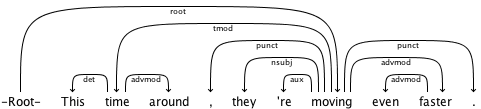
\includegraphics[width=1\linewidth]{gfx/nndep-example}
  \caption[Ejemplo de parseo de dependencias]{Ejemplo de parseo de dependencias}
  \label{fig:nndep}
\end{figure}

\begin{figure}[bth]
\makebox[\textwidth][c]{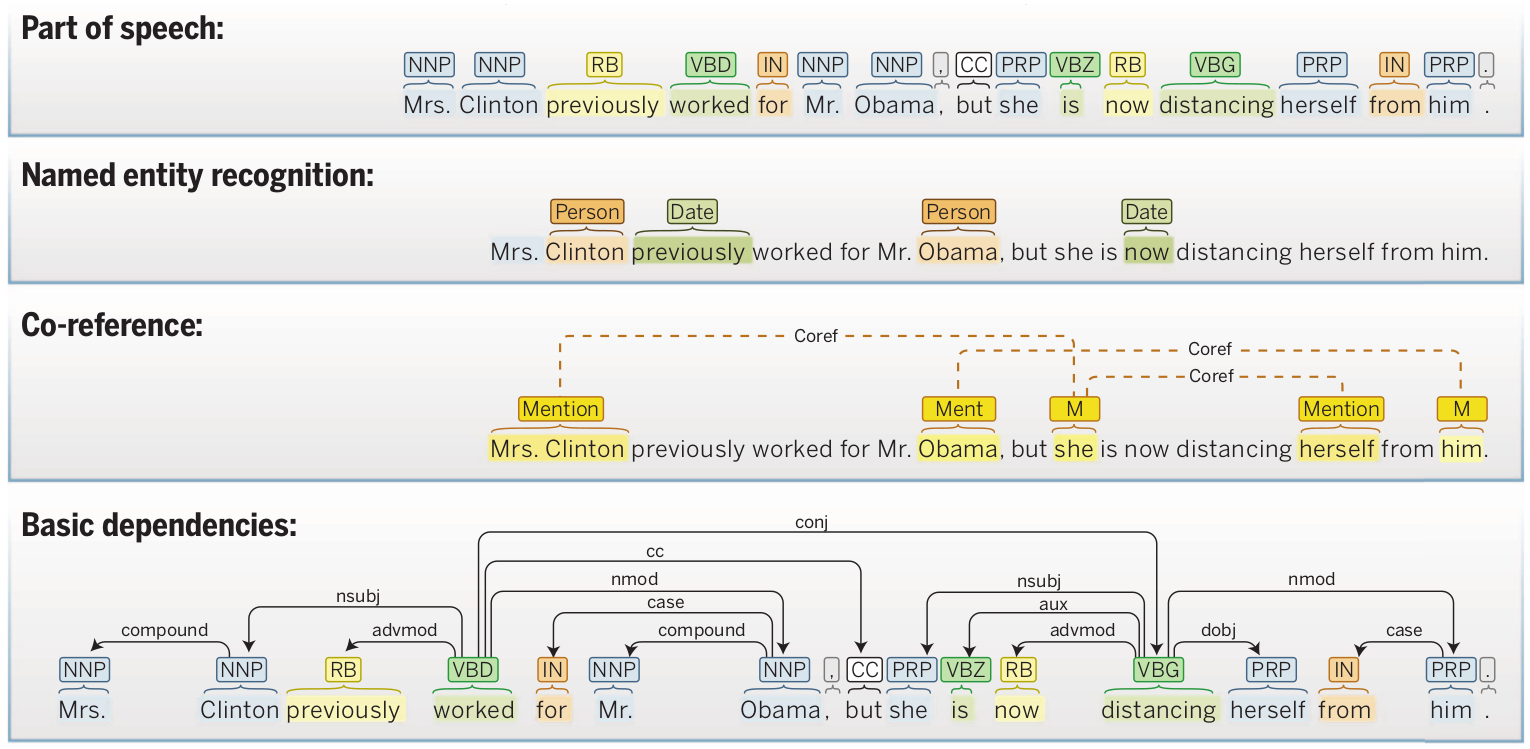
\includegraphics[width=1.5\textwidth]{gfx/corenlp}}
  \caption[Ejemplo de parseo de dependencias]{Many language technology tools
start by doing linguistic structure analysis. Here we show output from Stanford
CoreNLP. As shown from top to bottom, this tool determines the parts of speech
of each word, tags various words or phrases as semantic named entities of
various sorts, determines which entity mentions co-refer to the same person or
organization, and then works out the syntactic structure of each sentence, using
a dependency grammar analysis.}
  \label{fig:corenlp}
\end{figure}

\section{Limitaciones}
\label{sec:nlplimits}

Aunque se han producido avances, una de las principales limitaciones del
\ac{NLP} hoy día es el hecho de que la mayoría de recursos y sistemas solo están
disponibles para los denominados \emph{\acp{HRL}}\graffito{\ac{HRL}: Idiomas de
  altos recursos}, estos lenguajes son el Inglés, Francés, Español, Alemán y
Chino. Por contra, hay una gran cantidad de \emph{\acp{LRL}}
--\graffito{\ac{LRL}: Idiomas de bajos recursos} como Bengalí, Indonesio,
Punjabí, Cebuano y Swahili -- hablados y escritos por millones de personas que
no disponen de este tipo de sistemas. Uno de los mayores retos para la comunidad
del lenguaje es desarrollar recursos y herramientas para cientos o miles de
lenguajes, no solo para unos pocos.

Aún existiendo bastante \emph{software} trabajando con \ac{NLP}, y para idiomas
\ac{HRL}, suelen obtenerse mejores resultados para un idioma en concreto, el
Inglés. \change{Me dijiste ``\emph{justificar el por qué hemos decidido afrontar
    este problema}'', pero no se me ocurre qué poner} Es por ello que este
trabajo se ha centrado en desarrollar una fase del \emph{pipeline} que se
encuentra en todos los sistemas que realizan análisis de sentimientos, y en
general \ac{NLP} para el idioma Español. Como ejemplo podemos citar el famoso
\textsc{CoreNLP} \cite{manning-EtAl:2014:P14-5}.

En la \autoref{table:corenlpfeatures} se lista todo el \emph{pipeline} de
\textsc{CoreNLP} junto con el soporte para cada lenguaje. Como se aprecia, el
\emph{pipeline} esta completo únicamente para el Inglés. El objetivo de este
trabajo ha consistido en implementar un parseo de dependencias para el Español.

\newcommand*{\checktikz}[1][]{\tikz[x=1em, y=1em]\fill[#1] (0,.35) -- (.25,0) --
  (1,.7) -- (.25,.15) -- cycle;}

\newcommand*{\ccheck}{\checktikz[rounded corners=.5pt, draw=black,
  thin]} %\checktikz[rounded corners=.5pt, draw=red, ultra thin]

\begin{table}[]
  \centering
  \caption{\emph{Pipeline} de \textsc{CoreNLP} y disponibilidad por lenguaje}
  \label{table:corenlpfeatures}
  \begin{tabular}{lllllll}
    \rowcolor[HTML]{443627} 
    \multicolumn{1}{c}{\cellcolor[HTML]{443627}{\color[HTML]{FFFFFF} \textbf{ANNOTATOR}}} & \multicolumn{1}{c}{\cellcolor[HTML]{443627}{\color[HTML]{FFFFFF} \textbf{AR}}} & \multicolumn{1}{c}{\cellcolor[HTML]{443627}{\color[HTML]{FFFFFF} \textbf{ZH}}} & \multicolumn{1}{c}{\cellcolor[HTML]{443627}{\color[HTML]{FFFFFF} \textbf{EN}}} & \multicolumn{1}{c}{\cellcolor[HTML]{443627}{\color[HTML]{FFFFFF} \textbf{FR}}} & \multicolumn{1}{c}{\cellcolor[HTML]{443627}{\color[HTML]{FFFFFF} \textbf{DE}}} & \multicolumn{1}{c}{\cellcolor[HTML]{443627}{\color[HTML]{FFFFFF} \textbf{ES}}} \\
    Tokenize / Segment & \ccheck & \ccheck & \ccheck & \ccheck &  & \ccheck \\
    Sentence Split & \ccheck & \ccheck & \ccheck & \ccheck & \ccheck & \ccheck \\
    Part of Speech & \ccheck & \ccheck & \ccheck & \ccheck & \ccheck & \ccheck \\
    Lemma &  &  & \ccheck &  &  &  \\
    Named Entities &  & \ccheck & \ccheck &  & \ccheck & \ccheck \\
    Constituency Parsing & \ccheck & \ccheck & \ccheck & \ccheck & \ccheck & \ccheck \\
    Dependency Parsing &  & \ccheck & \ccheck & \ccheck & \ccheck &  \\
    Sentiment Analysis &  &  & \ccheck &  &  &  \\
    Mention Detection &  & \ccheck & \ccheck &  &  &  \\
    Coreference &  & \ccheck & \ccheck &  &  &  \\
    Open IE &  &  & \ccheck &  &  & 
  \end{tabular}
\end{table}

Con la introducción del \emph{pipeline} de \textsc{CoreNLP}, se pasa ahora a
describir el proceso que todo sistema para \ac{NLP} debe seguir. Comenzaremos
mencionando un proceso genérico, para después profundizar en el \emph{pipeline}
de un \emph{software} especícifo, \textsc{CoreNLP} en nuestro caso.

\section{El pipeline genérico}
\label{sec:genericpipeline}


